\title{SE2 CheatSheet}
\author{dthoma}
\date{August 2017}

\documentclass[a4paper, fontsize=6pt]{scrartcl}
\usepackage{multicol}
\usepackage{calc}
\usepackage{ifthen}
\usepackage[landscape]{geometry}
\usepackage{hyperref}
\usepackage{graphicx}
\usepackage{mathtools}
\usepackage{gensymb}
\usepackage{minted}
\usemintedstyle{bw}
\usepackage{ragged2e} 
\usepackage[T1]{fontenc}
\usepackage[utf8]{inputenc}
\usepackage{amsbsy}
\usepackage{amsfonts}
\usepackage{varwidth,pst-tree,pst-eps}
\usepackage{comment}
\usepackage{xcolor}

\usepackage{fontspec}

\setromanfont[
Path=fonts/Roboto/,
BoldFont=Roboto-Bold.ttf,
ItalicFont=Roboto-Italic.ttf,
BoldItalicFont=Roboto-BoldItalic.ttf
]{Roboto-Regular.ttf}
\setmonofont[
Path=fonts/Hack/,
BoldFont=Hack-Bold.ttf,
ItalicFont=Hack-Italic.ttf,
BoldItalicFont=Hack-BoldItalic.ttf
]{Hack-Regular.ttf}

%German-specific commands
%--------------------------------------
\usepackage[german]{babel}
%--------------------------------------

\graphicspath{ {images/} }

\AtBeginEnvironment{minted}{%
  \renewcommand{\fcolorbox}[4][]{#4}}

% This sets page margins to .5 inch if using letter paper, and to 1cm
% if using A4 paper. (This probably isn't strictly necessary.)
% If using another size paper, use default 1cm margins.
\geometry{top=0.5cm,left=0.5cm,right=0.5cm,bottom=0.5cm}

% Turn off header and footer
\pagestyle{empty}
 

% Redefine section commands to use less space
\makeatletter
\renewcommand{\section}{\@startsection{section}{1}{0mm}%
    {-1ex plus -.5ex minus -.2ex}%
    {0.5ex plus .2ex}%x
    {\normalfont\large\bfseries}}
    
\renewcommand{\subsection}{\@startsection{subsection}{2}{0mm}%
    {-1explus -.5ex minus -.2ex}%
    {0.5ex plus .2ex}%
    {\normalfont\normalsize\bfseries}}
    
\renewcommand{\subsubsection}{\@startsection{subsubsection}{3}{0mm}%
    {-1ex plus -.5ex minus -.2ex}%
    {1ex plus .2ex}%
    {\normalfont\small\bfseries}}
    
\makeatother

% Define BibTeX command
\def\BibTeX{{\rm B\kern-.05em{\sc i\kern-.025em b}\kern-.08em
    T\kern-.1667em\lower.7ex\hbox{E}\kern-.125emX}}

% Don't print section numbers
%\setcounter{secnumdepth}{0}


\setlength{\parindent}{0pt}
\setlength{\parskip}{0pt plus 0.5ex}


% -----------------------------------------------------------------------

\begin{document}

\footnotesize
\begin{multicols*}{5}


% multicol parameters
% These lengths are set only within the two main columns
%\setlength{\columnseprule}{0.25pt}
\setlength{\premulticols}{1pt}
\setlength{\postmulticols}{1pt}
\setlength{\multicolsep}{1pt}
\setlength{\columnsep}{2pt}

Von dthoma.

\section{Projektplanung}

Kein Wasserfall-Modell, sondern \textbf{Agil} (Scrum, XP) oder \textbf{Iterativ} (RUP, Spiral Development).

\subsection{Zeitaufteilung}

Inception (10d) - Elaboration (8w 3i) - Construction (22w 11i) - Transition (6w 3i).

\subsection{End of Elaboration}

Anforderungen (Requirements), Funktionsumfang (Scope), UI-Design, Software Architecture, IDE, Arbeitspakete.

\subsection{Anforderungen / Use Cases}

Bevor man die Arbeitsaufteilung machen kann (insbesondere wenn das Team geografisch verteilt ist) muss der \textbf{Scope} und die \textbf{Architektur} klar sein.

Use Cases sind grösser als User Stories:

Use Case: An der Kasse bezahlen

User Story: als ein Kunde will ich...

User Story: als Kassierer will ich...

\subsubsection{Inhalt}

ID, Beschreibung, Akzeptanz-Kriterien, Schätzung Aufwand, Priorität für Kunde, geleistete Stunden, Status, Kategorie

\subsubsection{Grösse}

Maximal \textbf{50-70\%} von dem, was eine Person in einer Iteration schafft. Idee: das Arbeitspaket sollte innerhalb der Iteration fertig werden.

\subsubsection{Organisation}

Sie müssen an einem Ort \textbf{zentral} gespeichert sein, von allen eingesehen und editiert werden können, \textbf{priorisierbar} sein, und sowohl Schätzungen als auch Ist-Zeiten (\textbf{Zeitaufschreibung}) enthalten.

Es soll genug Arbeitspakete geben, damit alle im Team während der nächsten Iteration \textbf{beschäftigt} sind. Genau soviele Arbeitspakete wie die Schätzungen zulassen, sodass sie auch innerhalb der Iteration fertig werden. Innerhalb des Teams werden die Arbeitspakete dann eigenverantwortlich zugeordnet, evtl. auch dynamisch verteilt. 

\begin{itemize}
    \item Entwickler schätzen Aufwand
    \item Kunde priorisiert Arbeitspakete
\end{itemize}

Einzige \textbf{Ausnahme}: architekturrelevante Arbeitspakete können vom System-Architekten in bestimmte Iterationen gesetzt werden, weil sonst das System nicht schlau gebaut werden könnte. Dies muss aber dem Kunden erklärt werden und der Kunde muss es absegnen.

\subsubsection{Fallstricke}

Nicht nur generische Arbeitspakete aufführen (Generisch: Domainmodell, Use Cases. Nicht-generisch: Funktionalität für Speichern des Warenkorbs), unproduktive Tätigkeiten aufführen (z.B. Serversetup), "abhakbar" schreiben.

\section{Projekt-Automation}

Alle Aufgaben, die mehrmals durchgeführt werden, sollten automatisiert werden.

\textbf{CRISP} (Complete, Repeatable, Informative, Scheudlable, Portable) inkl. Dependency Management, Performance (Parallelisierung, inkrementell) und Erweiterbarkeit (z.B. LESS Processing).

\subsection{Build Tools}

\textbf{Imperative (make):} Sehr mächtig, aber komplex, schwieriges Wiederverwenden und viel Copy \& Paste.

\textbf{Deklarative (maven):} Convention over configuration was zu kürzeren Buildfiles führt, wiederverwendbare Logik (Plugins), automatisiertes Dependency Management, jedoch weniger flexibel und gibt Projektstruktur vor.

\textbf{Moderne Tools (gradle, Apache buildr):} Bestes aus beiden Welten.

\subsection{Continuous Integration (CI)}

Always have a runnable product, Have fast feedback in case of errors, Allow division of work without losing control. Daily Build / Nightly Build: Alle 24h weil Buildzeit (inkl. Test) > 6h, "Daily Build": Alle 3h weil Buildzeit ~1h, mehr Entwickler => mehr Buildfehler: Teilsysteme entkoppeln damit weniger Entwickler am Gleichen arbeiten.

\section{Software Engineering Practices}

\subsection{Requirement Practices}

\textbf{Dig for requirements:} Zusammenarbeit mit dem Benutzer, denken aus Benutzersicht, kritisches Hinterfragen und Nachbearbeiten, genügend generell und abstrakt, Verfolgung des Ursprungs.

\textbf{Make quality a requirement:} z.B. max. Antwortzeiten, min. Datenmenge, Prüfung von Daten/Geräten. Oft schwierig zu ermitteln und doch wichtig, da bewusste Wünsche des Kunden.

\textbf{Deal with changes:} Änderungen an den Requirements einplanen, genügend abstrakt definieren, design for change, kurze Iterationen mit User Feedback.

\subsection{Design Practices}

\textbf{Don't repeat yourself:} benannte Konstanten, gemeinsam genutzte Funktionen statt Copy/Paste, Kommentare geben nur relevante Zusatzinformationen, Konfigurationsdaten in externen Files.

\textbf{Archieve orthogonality:} Keine Kopplung zwischen konzeptionell unabhängigen Aspekten. Nicht mehrere unabhängige Aufgaben als eine Routine, nicht mehrere unabhängige Abstraktionen als ein Objekt (Eliminate side effects between unrelated things), denn das Ziel ist eine hohe Kohäsion, Reduktion der Kopplung und möglichst wenig Abhängigkeiten.

\textbf{Design to test:} Testbarkeit vor Entwicklungszeit betrachten, die Testbarkeit hat Einfluss auf die Architektur. Evtl. gewisse Freiheitsgrade für Dependency Injection. Es kann das Design komplexer als produktiv nötig machen:

\begin{itemize}
    \item \textbf{Fake}: Vereinfachte, schnellere Implementierung (z.B. In-Memory DB).
    \item \textbf{Mock}: Auf Testfall zugeschnitten, prüft Reihenfolge und Inhalt der erwarteten Aufrufe.
    \item \textbf{Stub}: Auf Testfall zugeschnittene Antworten.
    \item \textbf{Dummy}: Objekte die nur herumgereicht, aber nie inspiziert werden.
\end{itemize}

\subsection{Implementation Practices}

\textbf{Fix broken windows:} Probleme beheben, wenn sie entstehen.

\textbf{Refactor early and often:} "Heilungsprozess", konstanter Verbesserungsprozess während wachsendem SW-Projekt.

\textbf{Vermeide "Programming by Coincidence/Luck":} Klares Ziel sehen und Design verfolgen. Nur auf spezifizierte Features von Libraries verlassen. Eingesetzte Technologien beherrschen. Annahmen dokumentieren und mit Assert \& Tests prüfen.

\subsection{Verification Practices}

\textbf{Test rigorously:} Früh, häufig und automatisch testen.

\textbf{Find issues once:} gefundene Fehler verstehen und dafür Test schreiben.

\textbf{Perform reviews:} In Sitzung oder selbständig, Findings festhalten (Severity, Action, Verantwortlicher).

\section{Error Handling Design}

\textbf{Fehler-Prävention:} Design \& Code Reviews. Testing, Static Analysis, Error Handling Design, Concurrency Design \& Testing.

\textbf{Defensive Programmierung:} Alle Werte von externen Quellen prüfen.

\textbf{Fehler-Barrikaden:} Barrikade - dahinter sind Werte gültig. Auf Klassenniveau heisst das, dass public Methoden Eingaben prüfen und private Methoden von geprüften Eingaben ausgehen.

\textbf{Fehlerbehandlung:} Konservativ (Fehlermeldung, Shutdown) oder Optimistisch (Neutrales Resultat, nächstmögliches Resultat, Warnung loggen)

\textbf{Korrektheit:} niemals ungenaues Resultat liefern.

\textbf{Robustheit:} Versuche Software am Laufen zu halten.

\textbf{Exeptions:} Für mögliche produktive Fälle, sicherheitsrelevante Fehler und in Java Throwable Error für nicht zu behandelnde Fälle.

\textbf{Assertions:} Für Programmierfehler, die nicht eintreten soillten, Post- und Preconditions. Assertions sind primär eine Stütze während der Entwicklung, und formale Kommentare.

\section{Design by Contract (DBC)}

Ein Vertrag legt Rechte (benefits) und Pflichten (obligations) zweier Parteien statt. Durch Bertrand Meier zur Designmethode entwickelt, DBC ist Teil seiner Programmiersprache ''Eiffel''. Für Methoden (Pre- und Postconditions) und Klassen (Klasseninvariante, muss vor und nach jedem Methodenaufruf erfüllt sein).

\subsection{Cofoja}

\begin{minted}{java}
@Invariant({
  // Pre- und Post-Bedingungen
  // für alle Funktionen
})
public interface PrimitiveIntStack {

@Requires ({ "!isFull()" })
@Ensures({ 
  "top() == value",
  "!isEmpty()"
})
void push(int value);

@Requires ({ "!isEmpty()" })
@Ensures({ 
  "result == old(top())",
  "!isFull()"
})
void pop();

// Pure
@Requires ({ "!isEmpty()" })
int top();

// Pure
boolean isEmpty();

// Pure
boolean isFull();
}

\end{minted}

\subsection{Conditions}

\textbf{Precondition:} Bedingungen die vor dem Aufruf erfüllt sein müssen.

\textbf{Postcondition:} Bedingungen die nach dem Aufruf erfüllt sein müssen.

\textbf{Invariant:} Bedingungen die immer erfüllt sein müssen.

\textbf{Pure:} Read-only Methoden

\textbf{Subtyp:} Ein Subtyp darf Preconditions lockern aber NICHT verschärfen, Postconditions verschärfen aber NICHT lockern und Invarianten verschärfen, aber nicht lockern.

\section{Story Splitting}

\subsection{Aufteilung Projekte}

Kein Projekt über eine Million, kein Projekt länger als 9 Monate. Bei zu grossen Projekten nach Kunden-Domäne und Geschäftsprozess aufteilen.

\subsection{Aufteilung Arbeitspakete}

Von der Basis-Version zur Vollausstattung: erst alles nice-to-have weglassen, später inkrementell mehr implementieren. Also nicht das perfekte Rad, dann die perfekte Achse und in 5 Jahren ein Auto liefern; sondern erst ein Skateboard, ein Motorrad und irgendwann ein Auto liefern.

Ideale Grösse von Arbeitspaketen:

\begin{itemize}
    \item Durchschnitt: was 1 Person in 1/4 eines Sprints schafft
    \item Maximum: was 1 Person in 50-70\% eines Sprints schafft
\end{itemize}

\begin{center}
\begin{tabular}{ |c|c|c| } 
 \hline
 Winziges Projekt & Kleines Projekt & Mittleres Projekt \\ 
 \hline
  & 8 Epics & 12 Epics \\ 
 50 User Stories & 120 User Stories & 200 User Stories \\ 
 \hline
\end{tabular}
\end{center}

\section{Testen in grösseren Projekten}

\subsection{Testtypen}

\textbf{Microtesting:} Isoliert und schnell (Mocking / Faking) einzelne Methoden testen, selten grosse Klassen. In unteren Architekturlayern. Schwachstellen: Testabdeckung sagt wenig aus, Testen in Isolation zeigt Fehler bei Integration nicht \& müssen bei strukturellem Refactoring neu geschrieben werden.

\textbf{Externe Systeme:} File-Synchronisation via FTP. Mocken? eher nicht, besser einen Linux-Laptop hinstellen und Testszenarien durchspielen

\textbf{Integrationstest:} Unit Tests ''auf den oberen Etagen'' von direkt unterhalb UI bis hinunter zur Datenbank, dort müssen dann zuerst die richtigen Testdaten eingeschoben werden. Integrationstests testen realistischere Szenarios, entdecken mehr Fehler, sind langliebiger, können teilweise UI Testing ersetzen, können jedoch mehr Zeit benötigen. Drittsysteme werden gemockt / gefaked.

\textbf{Systemtest:} Kompletter Test des Systems bei jedem Release: Regressiontest: funktioniert alles noch so wie vorher?, Performancetest, Browser-Kompatibilitätstest. 

\textbf{User Acceptance Test (UAT):} Änlich wie Systemtest aber mit Einbezug von Kunden, formale Abnahme.

\subsection{Testabdeckung}

\textbf{Anweisungabsdeckung (Statement Coverage):} Zähler an jeder Anweisung.

\textbf{Zweigabdeckung (Branch Coverage):} Jeder Zweig, welcher durch die Unit Tests ausgeführt wird zählt. Abweichung zu Anweisungsabdeckung: If ohne else mit Testfall, wo das IF grad ganz ausgelassen wird, For und while Testfälle, bei denen man garnicht in die Schleife geht.

\textbf{Bedingungsabdeckung (Decision Coverage):} Alle Kombinationen von Bedingungen, welche zum Eintritt in einen Block führen müssen getestet werden. Das Verhältnis von ausgewerteten atomaren Werten zu allen vorhandenen atomaren Werten. Kann hilfreich sein, Testdaten mit Äquivalenzklassen selektieren.

\textbf{Pfadabdeckung (Path Coverage):} Jede mögliche Kombination von Zweigen ist abgedeckt. Das Verhältnis der getesteten Pfade zu allen möglichen Pfaden in einem Modul. Führt sehr schnell zu einer potentiell unendlichen Anzahl von Fällen (wegen Schleifen).

\subsection{Server-Umgebung}

\begin{tabular}{|p{0.1\linewidth}|p{0.7\linewidth}|}
 \hline
 PROD & stabile, produktive Umgebung, keine Experimente \\ 
 \hline
 ACC & Acceptance (auch STAGE), manuelles Testen durch Kunde, möglichst produktionsnah, für Performance-Tests. \\ 
 \hline
 TEST & Stabile Test Umgebung für Entwickler, automatisierte Tests, einzelne Performance Tests, Deployment nach Sprint Ende. \\ 
 \hline
 DEV & Entwicklungssystem, Daily Build \\ 
 \hline
\end{tabular}


\section{Aufwandschätzung}

\subsection{Faktoren}

\textbf{Nicht Linear:} Communication, Planning, Management, Requirements development, System functional design, Interface design and specification, Architecture, Integration, Defect removal, System testing, Document production

=> Keep it small. Schätzen ist Erfahrungssache

\subsection{Top Down Schätzung}

Vor allem zu begin der Elaboration:

\begin{enumerate}
    \item Modell wählen z.B. COCOMO (berücksichtigt Projektgrösse + Einflussfaktoren)
    \item Schätzung durchführen
    \item Nach Projektende: geschätzte Zeit mit tatsächlichem Aufwand vergleichen
    \item Modell kalibrieren (Parameter anpassen)
\end{enumerate}

\subsection{Bottom Up Schätzung}

Nach Elaboration, wenn alle Requirements bekannt sind und ein vorläufiger Entwurf vorhanden ist (Architektur, Design, Tools).

Liste aller Artbeiten (codieren, GUI, Daten-Entwurf), Nicht Programmier Aufgaben (Testing, Dokumentation, Sitzungen, ...), Alle Elemente einzeln schätzen

\subsection{Algorithmische Modelle}

\subsubsection{COCOMO}

KDSI: K delivered source instructions (1000 Zeilen Code)

Person-Months (PM) $$ PM = 3.2 * (KDSI) ^{1.05} $$ Development Time: $$ 2.5 * (PM)^{0.38} $$

\subsubsection{LOC}

100 - 1000 ausgelieferte Zeilen Code / Person \& Monat. Wenn man keine anderen Erfahrungswerte hat, dann 400 DLOC annehmen (pro Monat und Entwickler).

\section{Metriken}

\subsection{Zyklomatische Zahl}

Misst Komplexität der logischen Struktur auf Basis Kontrollflussgraph G eines Programms. Zyklomatische Zahl (Anzahl linear unabhängiger Pfade durch Programm). $G$ berechnet sich $V(G) = e -n + 2p$ mit der Anzahl Kanten (edges) $e$, Anzahl Knoten (nodes) $n$ und Anzahl Komponenten (unabhängige Teil-Graphen) $p$. Für einzelne Funktion/Methode kann die vereinfachte Formel $V(G) = Anzahl Verzweigungen + 1$ verwendet werden.

\textbf{Faustregel:} $V(G)$ einer Funktion / Methode > 10 => Methode / Funktion genauer anschauen.

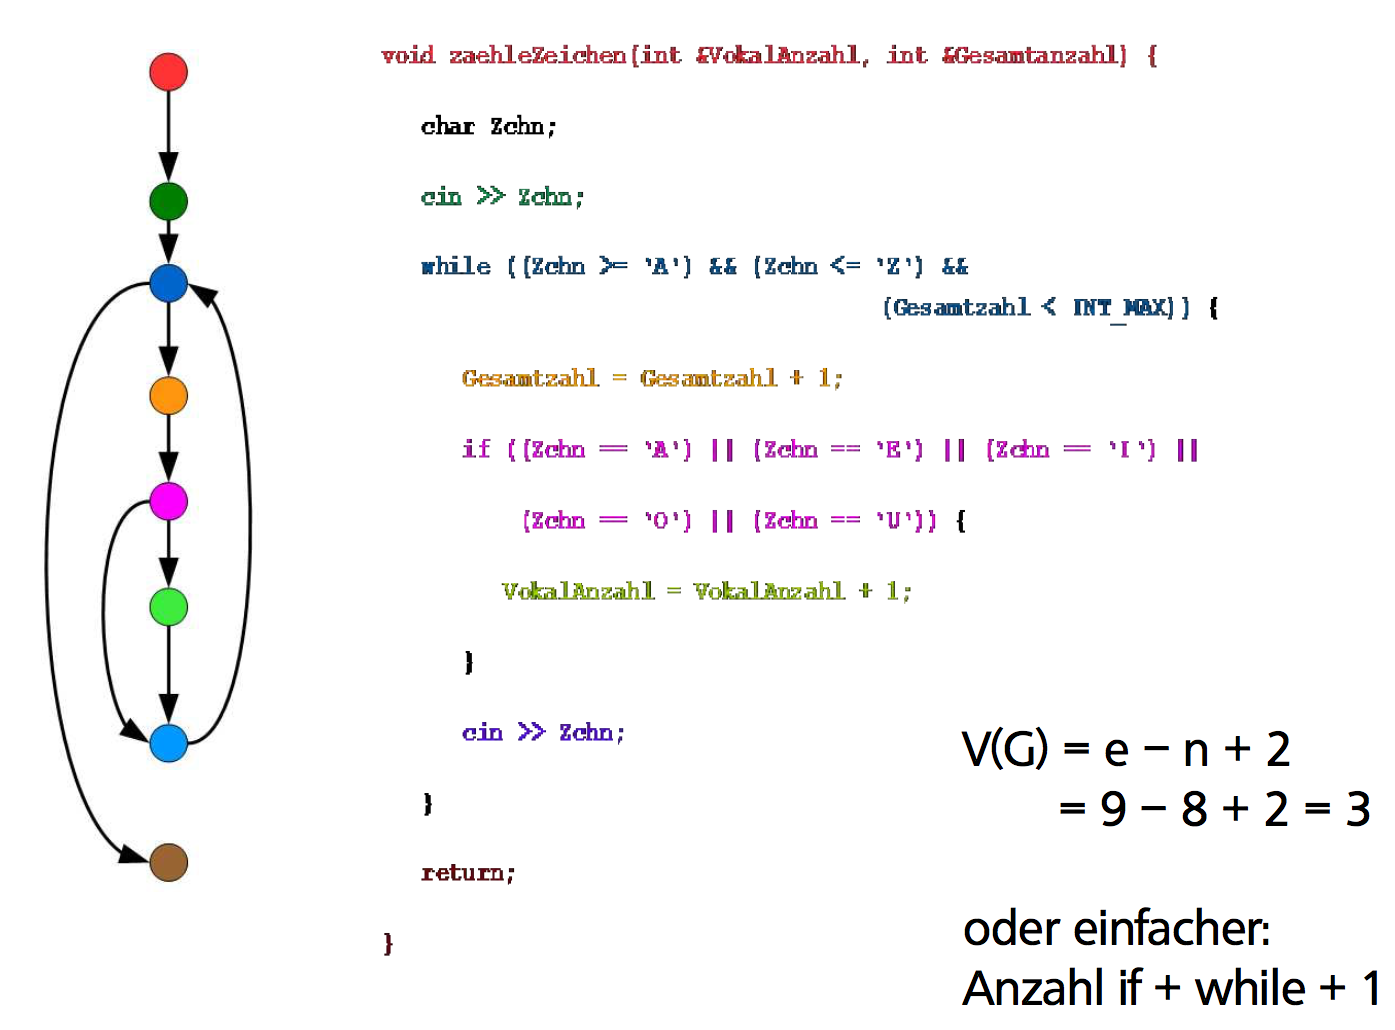
\includegraphics[scale = 0.11]{kontrollflussgraph.png}

\begin{center}
\begin{tabular}{ |c|c|c| }
\hline
 1-10 & simple, without much risk \\ 
 11-20 & more complex, moderate risk \\  
 21-50 & complex, high risk program \\
 > 50 & untestable program (very high risk) \\
\hline
\end{tabular}
\end{center}

\subsection{Lack of Cohesion of Methods (LCOM)}

$$LCOM = \frac{m-Mittelwert((m(A))}{m-1}$$

$m$ Anzahl Methoden, $m(A)$ Anzahl Methoden, die auf ein Attribut zugreifen, $Mittelwert(m(A))$ über alle Attribute. Getter und Setter verschlechtern LCOM (Benutzen nur ein Attribut).

\textbf{Beispiel:} Jede Methode greift nur auf ein Attribut zu -> $LCOM = 1$ -> schlechte Kohäsion, jede Methode greift auf alle Attribute zu, einfacheres Refoctoring  -> $LCOM = 0$ -> gute Kohäsion

\subsection{Instability (I)}

\textbf{Afferent Coupling} $C_a$ Anzahl Klassen ausserhalb eines Packages, die von Klassen innerhalb des Packages abhängen.
\textbf{Efferent Coupling} $C_e$ Anzahl Klassen innerhalb des Packes, die von Klassen ausserhalb des Packages abhängen.

$$ I=\frac{C_e}{C_a+C_e} $$

Falls $I=1$ ist die Klasse instabil (Package am Rand. Falls $I=0$ ist die Klasse stabil (zentrales Package).

\subsection{Normalized Distance from Main Sequence (Dn)}

Abstractness $A$ = $$\frac{\text{Anzahl abstrakter Klassen}}{\text{Anzahl Klassen eines Packages}}$$

$$D_n=|A+I-1|$$

$D_n$ sollte bei gutem Package Design möglichst tief sein.

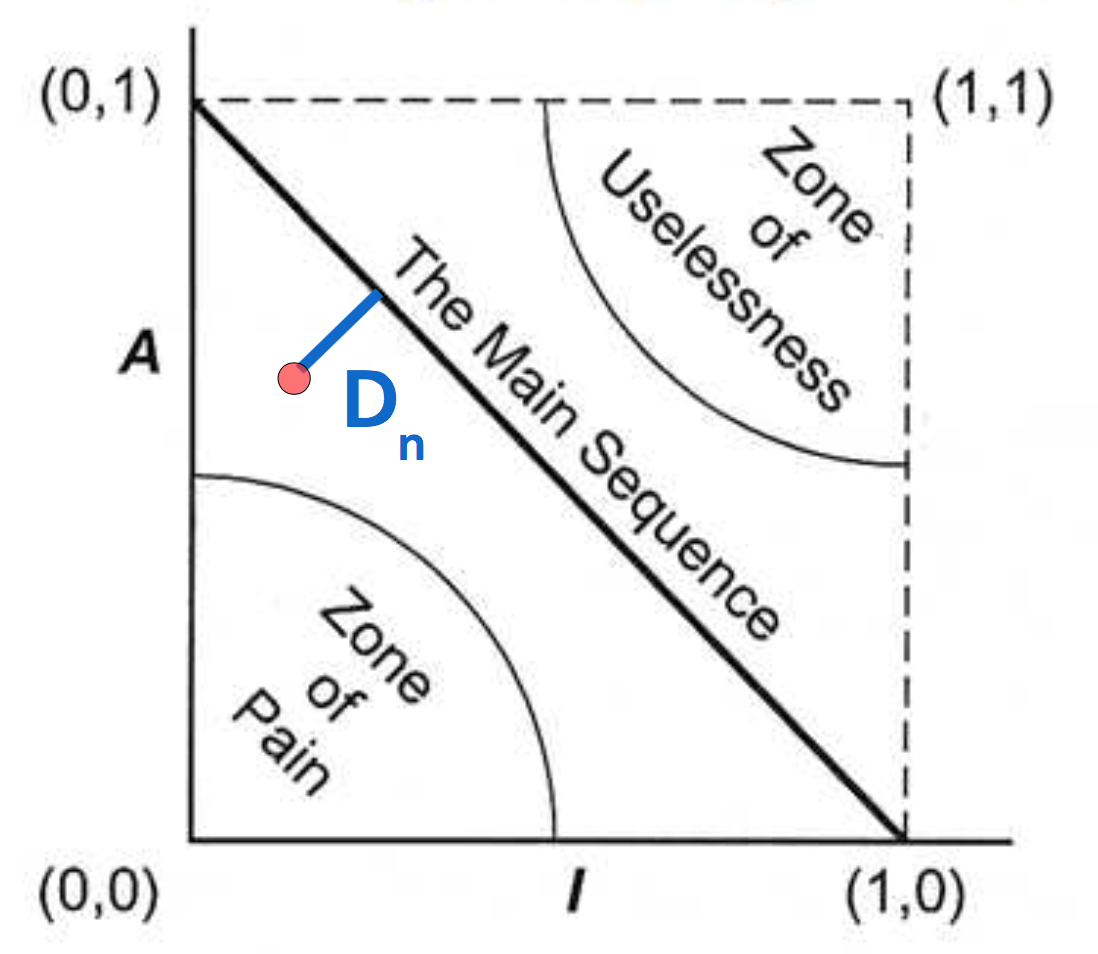
\includegraphics[scale = 0.14]{zoneof.png}
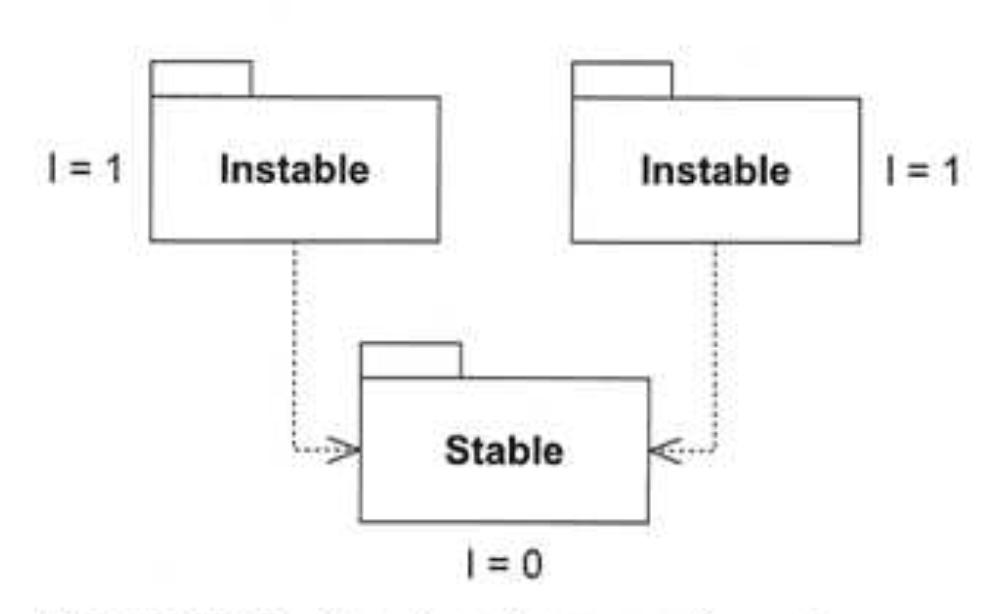
\includegraphics[scale = 0.14]{idealpackageconfiguration.png}

Refaktorisiert werden sollte das Package, welches am Weitesten von der Main-Sequence entfernt liegt. Die Kern-Applikation ist meist sehr Stabil und nahe bei der ''Zone of Pain'', da Sie wenige Abhängikeiten zu anderen Packages hat.

\subsection{Structure 101}

Visualisiert Abhängigkeiten mit Richtung und Anzahl Referenzen.

\section{Code Reviews}

Immer zwischen Peers aus der eigenen Abteilung mit Gruppe mehrerer Personen, definierten Rollen, definiertem Stück Code, begrenzter Zeit, Protokoll und Nacharbeiten.

\begin{enumerate}
    \item Frühe Fehlerentdeckung
    \item Team verbessert sich
    \item Know-How über Architektur verbreitet sich
    \item Reviews sind kosteneffizient
\end{enumerate}

\section{Performance Messungen}

\begin{itemize}
    \item Get it to run (Sunny Case)
    \item Get it right (robust, fehlerfrei)
    \item Make it fast (erst jetzt Performance)
\end{itemize}

Erst messen, dann optimieren. Problem mit Testdaten: NICHT random, sondern zum Beispiel populäre Artikel viel häufiger.

Der Java Profiler zeigt auf, welche Methode viel Rechenzeit benötigt.

\section{Usability Testing}

User sollten nicht vorbelastet sein. Dem User sollten die Aufgaben offen gestellt werden, ohne zu helfen und zu führen. \textbf{Wireframes} zeigen die Funktionalität, was man machen kann. \textbf{Mockups} zeigen, wie es aussehen wird (graphisches Design).

\section{Scrum 2}

\subsection{Product Owner VS. Projektleiter}

PO macht keine aktive Risiko-Beobachtung, PO macht normalerweise keine Stakeholderanalyse, PO hält den Scope nicht im Auge, PO kann Qualität nicht einschätzen.

\subsection{Impediments}

Impediment = Hindernis, das nicht innerhalb des Scrum Teams beseitigt werden kann. Beispiel: unperformantes 3rd Party System wird im Impediment Tracking festgehalten.

\subsection{MVP (Minimum Viable Product)}

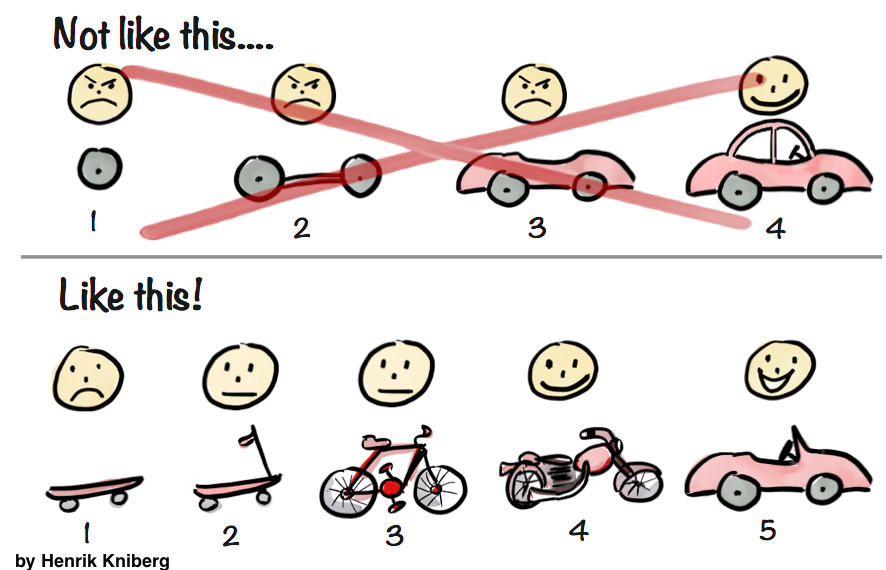
\includegraphics[scale=0.15]{minimal-viable-product-henrik-kniberg.png}

\section{Proving Programs Correct}

\subsection{Hoare Triples}

\begin{minted}{go}
{P}C {Q}
\end{minted}

P = Precondition \\
C = Command/Program \\
Q = Postcondition \\

If a program C is executed from an initial state satisfying the precondition P, the final state after C terminates, satifies the postcondition Q.

\begin{minted}{go}
{x = a ^ y = b}
t:=x;
x:=y;
y:=t;
{x = b ^ y = a}
\end{minted}

\subsection{Weakest Precondition}

\begin{minted}{go}
{x = a} => {x 1 3 = a + 3} <=> wahr
{x + 3 = a + 3}
x :=x + 1
{x + 2 = a + 3}
x := x + 2
{x = a + 3}
\end{minted}

\begin{enumerate}
    \item von unten nach oben immer Variable mit Zuweisung ersetzen
    \item zum Beweisen, dass die Precondition stimmt beweisen dass, Precondition => berechnete Precondition
    \item (Mit gegebener Precondition vergleichen)
\end{enumerate}

\subsection{if}

\begin{minted}{go}
{T}
// {(cond => b && !cond => a)}
{(x < 0 => -x >= 0)  && (!(x < 0) => x >= 0)}
if x < 0 then
    {-x >= 0} // b
    y := -x
else
    {x >= 0} // a
    y := x
{y >= 0}
\end{minted}

\begin{enumerate}
    \item Fallunterscheidung, einmal if erfüllt, einmal nicht.
    \item Beweisen \texttt{T => ((cond => b \&\& !cond => a))}
\end{enumerate}

\subsection{while}

\begin{minted}{go}
{x >= 0} // a: Precondition
{0 <= x} // b
i := 0
{i <= x} // c: Invariante
while i != x do {Inv: i <= x}
    {i <= x && i != x} // d: Inv & Cond
    {i + 1 <= x} // e
    i := i + 1
    {i <= x} // f: Invariante
{i <= x && !(x != i)} // g: Inv && (!Cond)
{i = x} // h
\end{minted}

\begin{enumerate}
    \item Invariante Inv bestimmen (Bedingung, die vor und nach jedem Schleifendurchgang erfüllt sein muss. Kann sein, dass mehrere ausprobiert werden müssen)
    \item Schleifen Vorbedingung c = Invariante
    \item Erste Bedingung in Schleife d = Invariante \&\& Schleifenbedingung
    \item Letzte Bedingung in Schleife f = Invariante
    \item Schleifen Nachbedingung g = Invariante \&\& !Schleifenbedingung
    \item e und b von Unten nach Oben berechnen
    \item Beweisen: \texttt{a=>b\&\&d=>e\&\&g=>h}
\end{enumerate}

Beweisen (z.B. $a => b$
$$\vdash a => b\\
$$
$b$ umformen/vereinfachen, bis $b \iff a$

\section{TDD}

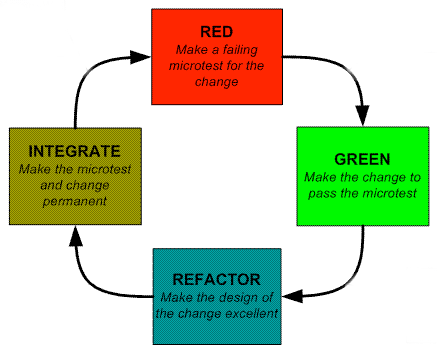
\includegraphics[scale=0.3]{tddcyclewithdesign.png}

\textbf{RED} heisst, neuer Test der Fehlschlägt, aber kompiliert und sollte nur wenige Minuten dauern.
\textbf{GRÜN} sollte unter 10 min stehen bleiben (copy-paste-status).

\subsection{TDD Patterns}

\textbf{Specify It}:

\textit{Essence First:}
XML: zuerst Open/Close a Tag, Attribute, innere Werte usw. später

\textit{Test First:}
\mintinline{java}{testSimpleOpenClosedTag() {}}

\textit{Assert First:}
Assertion zuerst schreiben (auch Client-Code zuerst schreiben), danach erst das Setup

\textbf{Frame It}

\textit{Frame First:}
Kompilierbar machen

\textbf{Evolve It}

\textit{Do The Simplest Thing That Could Possibly Work:}
Sometimes all you'll produce is a method that returns a hard-coded value. Never mind that.

\textit{Break It To Make:}
Nun schreibt man weitere Tests, zum Beispiel mit einem anderen erwarteten Wert. Erst dann baut man das ins Programm ein, so dass der Wert dynamisch ist.

\textit{Refactor Mercilessly}

\textit{Test Driving}

Immer kurze Schritte!

\section{Code Smells}

\begin{tabular}{|p{0.2\linewidth}|p{0.6\linewidth}|}
 \hline
 Code Smell & Beschreibung => Refactoring \\ 
 \hline
 Speculative Generality & Unbenutzte Klassen, Methoden, Attribute oder Parameter weil der Programmierer ''Just in Case'' Features eingebaut hat. => Collapse Hierarchy, Inline Class, Remove Parameter, Rename Method \\ 
 \hline
 Comment & Viele Kommentare statt gute Namen. => Extract Method, Rename Method \\ 
 \hline
 Long Method & Zu viele Codezeilen in Methode (> 10 Zeilen). => Extract Method, Replace Temp with Query, Introduce Parameter Object, Preserve Whole Object, Replace Method with Method Object \\ 
 \hline
 Long Parameter List & Mehr als 3 - 4 Parameter in Methode. => Replace Parameter with Method, Preserve Whole object, Introduce Parameter Object \\ 
 \hline
 Magic Numbers & Zahlenliterale statt Konstanten => Replace Magic Number with Symbolic Constant. \\ 
 \hline
 Duplicated Code & Zwei Codefragmente, die fast gleich aussehen oder das Gleiche machen => extract Method \\ 
 \hline
 Large Class & Zu viele Methoden, Attribute oder Codezeilen => Extract Class, Extract Subclass \\
 \hline
 Conditional Complexity & Komplizierte Bedingungen und lange if -Statements =>
wenn Fallunterscheidungen für verschiedene Berechnungen: Replace Conditional Logic with Strategy

wenn Fallunterscheidungen Zustandsübergänge eines Objekts kontrollieren: Replace State-Altering Conditionals with State

wenn Fallunterscheidungen für Zusatzfunktionalität: Move Embellishment (Ausschmückung) to Decorator

Wenn viele Fallunterscheidungne für Spezialfall "Objekt nicht vorhanden": Introduce Null Object
  \\ 
 \hline
 Switch / Case & Komplexe switch Statements oder if -Sequenzen => extract Method oder Replace Type Code with State/Strategy (besonders mit instanceOf()). \\ 
 \hline
 Primitive Obsession & (Abstraktionsebene zu tief) Verwendung von primitiven Typen statt Objekte für einfache Aufgaben (z.B. Währung, Ranges). => Replace Data Value with Object, Replace Type Code with Class/Subclass or State/Strategy Pattern, Extract Class \\ 
 \hline
 Oddball Solution & Verschiedene Lösungen für das Gleiche Problem. => Substitute Algorithm ODER Unify Interfaces with Adapter \\ 
 \hline
 Refused Bequest & Eine Klasse benutzt nur wenige der geerbten Methoden und Attribute (\textbf{Liskov} verletzt) => Replace Inheritance with Delegation, Push Down Method/Field \\ 
 \hline
 Inappropirate Intimacy & Eine Klasse verwendet interne Felder und Methoden einer anderen Klasse \textbf{auf Klassenebene} => Move Method und Move Field, vermutlich sind die Methoden in der falschen Klasse. \\ 
 \hline
 Indecent Exposure & Eine Klasse zeigt interne Felder und Methoden einer anderen Klasse \textbf{auf Package-Ebene}=> Encapsulate Classes with Factory ODER Dependency Injection \\ 
 \hline
 Feature Envy & Methode greift häufiger auf Daten einer anderen Klasse zu als auf die eigenen. => Move Method, Extract Method \\ 
 \hline
 Middle Man & Klasse, die nichts anderes macht als Arbeit an andere Klassen zu delegieren. => Remove Middle Man \\ 
 \hline
 Shotgun Surgery / Solution Sprawl & Änderungen haben oft viele kleine Anpassungen in verschiedenen Klassen zur Folge (auch von Duplicated Code aus). => Move Method und Move Field um Single Responsibility herzustellen ODER Move creation knowledge to factory \\ 
 \hline
\end{tabular}

\section{GRASP Patterns}

\textbf{Controller:} The controller pattern assigns the responsibility of dealing with system events to a non-UI class that represents the overall system or a use case scenario. A controller object is a non-user interface object responsible for receiving or handling a system event.
\textbf{Creator:} Creation of objects is one of the most common activities in an object-oriented system. Which class is responsible for creating objects is a fundamental property of the relationship between objects of par0rticular classes.
\textbf{High cohesion:} High cohesion is an evaluative pattern that attempts to keep objects appropriately focused, manageable and understandable. High cohesion is generally used in support of low coupling. High cohesion means that the responsibilities of a given element are strongly related and highly focused. Breaking programs into classes and subsystems is an example of activities that increase the cohesive properties of a system. Alternatively, low cohesion is a situation in which a given element has too many unrelated responsibilities. Elements with low cohesion often suffer from being hard to comprehend, hard to reuse, hard to maintain and averse to change.
\textbf{Indirection:} The indirection pattern supports low coupling (and reuse potential) between two elements by assigning the responsibility of mediation between them to an intermediate object. An example of this is the introduction of a controller component for mediation between data (model) and its representation (view) in the model-view-controller pattern.
\textbf{Information expert:} Information expert (also expert or the expert principle) is a principle used to determine where to delegate responsibilities. These responsibilities include methods, computed fields, and so on.
\textbf{Low coupling:} Coupling is a measure of how strongly one element is connected to, has knowledge of, or relies on other elements. Low coupling is an evaluative pattern that dictates how to assign responsibilities to support: lower dependency between the classes, change in one class having lower impact on other classes, higher reuse potential.
\textbf{Polymorphism:} According to polymorphism principle, responsibility of defining the variation of behaviors based on type is assigned to the type for which this variation happens. This is achieved using polymorphic operations. The user of the type should use polymorphic operations instead of explicit branching based on type.
\textbf{Protected variations:} The protected variations pattern protects elements from the variations on other elements (objects, systems, subsystems) by wrapping the focus of instability with an interface and using polymorphism to create various implementations of this interface.
\textbf{Pure fabrication:} A pure fabrication is a class that does not represent a concept in the problem domain, specially made up to achieve low coupling, high cohesion, and the reuse potential thereof derived (when a solution presented by the information expert pattern does not). This kind of class is called a ''service'' in domain-driven design.


\section{Refactorings}

\begin{tabular}{|p{0.2\linewidth}|p{0.6\linewidth}|}
 \hline
 Refactoring & Beschreibung \\ 
 \hline
 Replace Temp with Query & Temporäre Variable mit Methoden(aufruf) ersetzen \\ 
 \hline
 Extract Method & Komplizierter Ausdruck in Methode verschieben \\ 
 \hline
 Inline Method & Methodenbody in Code verschieben (Gegenteil von Extract Meth‡od) \\ 
 \hline
 Move Method & Methode in andere Klasse verschieben. \\ 
 \hline
 Move Field & Attribut in eine andere Klasse verschieben. \\ 
 \hline
 push down & Methode / Field von Parentklasse in Subklasse verschieben. \\ 
 \hline
 pull up & Methode / Field von Subklasse in Parentklasse verschieben. \\ 
 \hline
 Change Value to Reference & Vor allem in Sprachen wie C++, Value zu Referenz ändern. \\ 
 \hline
 Change Reference to Value & Vor allem in Sprachen wie C++, Referenz zu Value ändern. \\ 
 \hline
 Replace Magic Number with Symbolic Constant & Zahl Literal mit gut benannter Konstante ersetzen. \\ 
 \hline
 Change Method Signature & Methodenparameter entfernen oder Reihenfolge ändern. \\ 
 \hline
 Encapsulate Field & public Field private machen und getter / setter bereitstellen \\ 
 \hline
 Replace Type Code with Class & Wenn Verhalten nicht abhängig vom Typ => Type Code (typischerweise Int) mit Enum ersetzen. \\ 
 \hline
 Replace Type Code with Subclass & Verhalten der Klasse abhängig vom Typ-Attribut 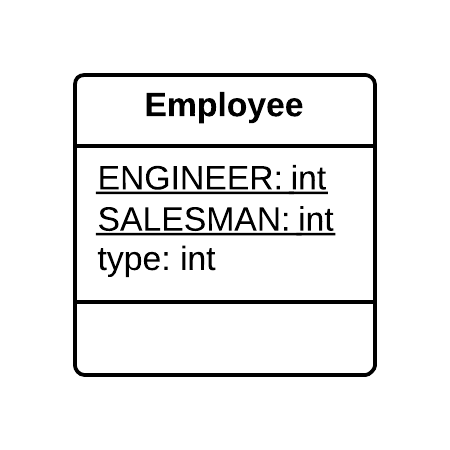
\includegraphics[scale=0.08]{ReplaceTypeCodeWithSubclassesBefore.png} 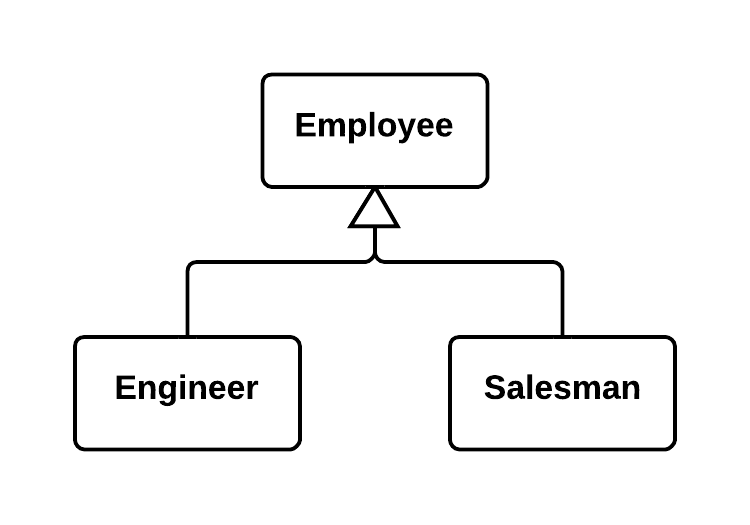
\includegraphics[scale=0.07]{ReplaceTypeCodeWithSubclassesAfter.png} \\ 
 \hline
 Replace Type Code with State / Strategy & Verhalten der Klasse abhängig vom Typ aber aus irgend einem Grund kann keine Subklasse verwendet werden, => State/Strategy Pattern\\
 & 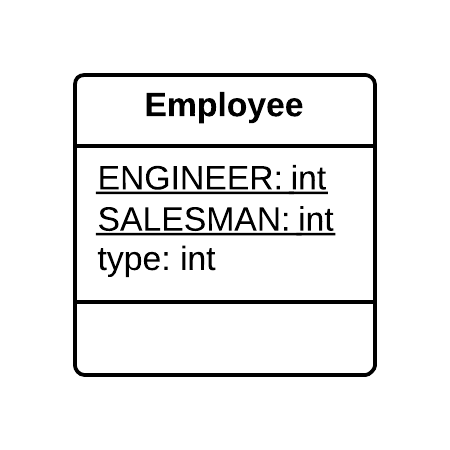
\includegraphics[scale=0.07]{ReplaceTypeCodeWithStateStrategyBefore.png}
 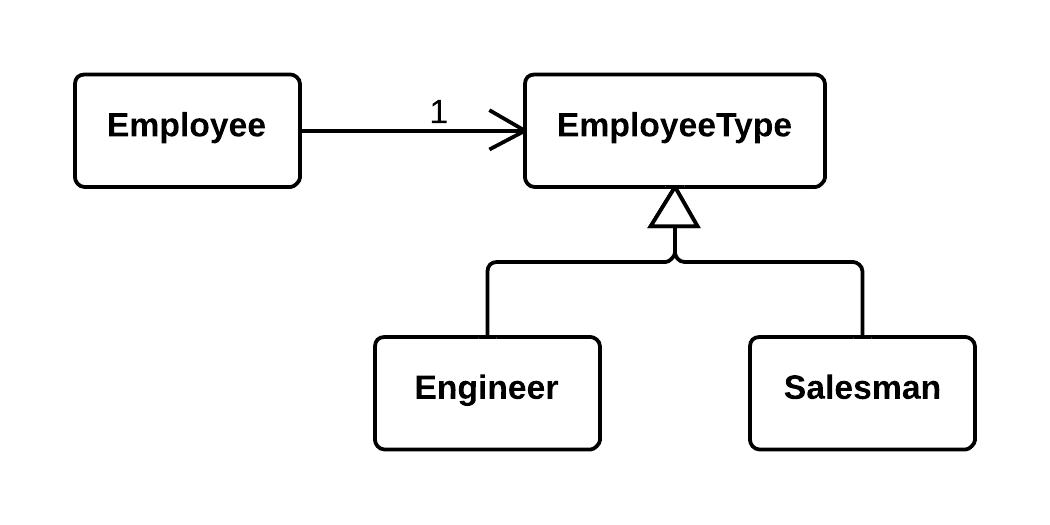
\includegraphics[scale=0.05]{ReplaceTypeCodeWithStateStrategyAfter.png}\\ 
 \hline
 Decompose Conditional & Bei kompliziertem if: Extract Methods für Bedingungen, if-Block und else- Block. \\ 
 \hline
 Replace Nested Conditional with Guard Clauses & Geschachtelte Bedingungen machen Normalablauf unübersichtlich => verwende für Spezialfälle Guards mit entsprechenden Methoden \\ 
 \hline
 Replace (Nested) Constructor with Factory Method & Constructor mit Factory Methode ersetzen. Oft nach Replace Type Code with Strategy nötig, Instanziere andere Subklasse, je nach Typ. \\ 
 \hline
 Replace Exception with Test & Statt bei invalidem Methodeninput eine Exception zu werfen soll der Aufrufer die Bedingung vor Methodenaufruf prüfen und nur aufrufen, wenn diese erfüllt ist. \\ 
 \hline
 \end{tabular}
 
 Continued
 
 \begin{tabular}{|p{0.2\linewidth}|p{0.6\linewidth}|}
 \hline
 Refactoring & Beschreibung \\ 
 \hline
 Extract Subclass & Erzeuge Unterklasse für Funktionen, welche nur von einzelnen Instanzen verwendet werden. \\ 
 \hline
 Extract Superclass & Erzeuge Basisklasse für Klassen mit ähnlichen Eigenschaften. \\ 
 \hline
 Extract Interface & Zwei Klassen verwenden gleiche Interfaces => neues Interface als Kombination aller Interfaces / Zwei Klassen verwenden nur Teile eines Interfaces => neues Interface mit den Teilen, die gebraucht werden. \\ 
 \hline
 Collapse Hierarchy & Basisklasse und Unterklassen unterscheiden sich nur wenig => Klassen zusammenfügen. \\ 
 \hline
 Replace Inheritance with Delegation & Vererbung mittels Delegation auflösen. \\ 
 \hline
 Substitute Algorithm (Fowler) & Algorithmus durch besser verständlichen ersetzen. \\ 
 \hline
 Unify Interfaces with Adapter (GOF) &  \\
 \hline
  Replace Conditional Logic with Strategy & Eine Strategy-Klasse für jede Variante erstellen, dann die Methoden der Strategy-Instanz aufrufen \\ 
  \hline
  Replace State Altering Conditionals with State & Bedingungen mit State-Klassen ersetzen, welche die spezifischen States und Übergänge behandeln\\
  \hline
  Move Embellishment (Ausschmückung) to Decorator & Move the embellishment code to a Decorator \\
  \hline
  Introduce Null Object & Spezielles Objekt erstellen, dass sich wie null verhält, aber nicht null selber ist (keine Nullpointer-Exceptions) \\ 
 \hline
  Replace Conditional Logic with Strategy & Create a Strategy for each variant and make the method delegate the calculation to a Strategy instance \\ 
 \hline
 Encapsulate Classes with Factory & Konstruktoren privat machen, Clients erstellen Instanzen über eine Factory  \\ 
 \hline
\end{tabular}

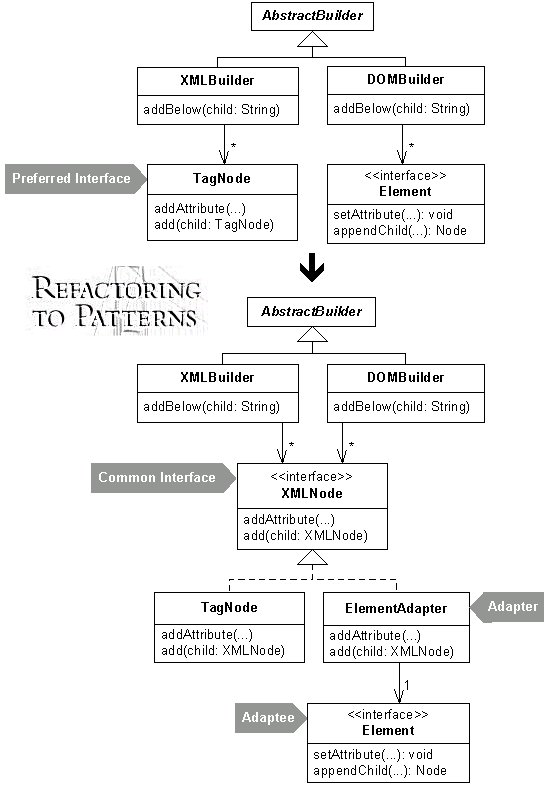
\includegraphics[scale=0.2]{interfacesWithAdapter.jpg}

\end{multicols*}
\end{document}
